\documentclass[compress]{beamer}
\usepackage{ifthen,verbatim}

\newcommand{\isnote}{}
\xdefinecolor{lightyellow}{rgb}{1.,1.,0.25}
\xdefinecolor{darkblue}{rgb}{0.1,0.1,0.7}

%% Uncomment this to get annotations
%% \def\notes{\addtocounter{page}{-1}
%%            \renewcommand{\isnote}{*}
%% 	   \beamertemplateshadingbackground{lightyellow}{white}
%%            \begin{frame}
%%            \frametitle{Notes for the previous page (page \insertpagenumber)}
%%            \itemize}
%% \def\endnotes{\enditemize
%% 	      \end{frame}
%%               \beamertemplateshadingbackground{white}{white}
%%               \renewcommand{\isnote}{}}

%% Uncomment this to not get annotations
\def\notes{\comment}
\def\endnotes{\endcomment}

\setbeamertemplate{navigation symbols}{}
\setbeamertemplate{headline}{\mbox{ } \hfill
\begin{minipage}{5.5 cm}
\vspace{-0.75 cm} \small
\end{minipage} \hfill
\begin{minipage}{4.5 cm}
\vspace{-0.75 cm} \small
\begin{flushright}
\ifthenelse{\equal{\insertpagenumber}{1}}{}{\hspace{0.2 cm} \Large \textcolor{darkblue}{\insertpagenumber\isnote/\pageref{numpages}}}
\end{flushright}
\end{minipage}\mbox{\hspace{0.2 cm}}\hspace{0.01 cm} \vspace{-1.05 cm}}

\begin{document}
\begin{frame}
\vfill
\begin{center}
\textcolor{darkblue}{\Large Fundamental Particles \\ \vspace{0.2 cm} and the Forces that Move Them}

\vfill
\begin{columns}
\column{0.3\linewidth}
\begin{center}
\large
Jim Pivarski
\end{center}
\end{columns}

\vfill
14 July, 2010
\end{center}
\end{frame}

%% \begin{notes}
%% \item This is the annotated version of my talk.
%% \item If you want the version that I am presenting, download the one
%% labeled ``slides'' on Indico (or just ignore these yellow pages).
%% \item The annotated version is provided for extra detail and a written
%% record of comments that I intend to make orally.
%% \item Yellow notes refer to the content on the {\it previous} page.
%% \item All other slides are identical for the two versions.
%% \end{notes}

\small

\begin{frame}
\frametitle{The basic idea: an analogy}
\begin{itemize}
\item Studying particle physics is like trying to figure out the rules
  of the universe's chess game
\item Other sciences study game-strategies using rules we already know
\item But there's still more to learn about the basic rules
\end{itemize}

\begin{center}
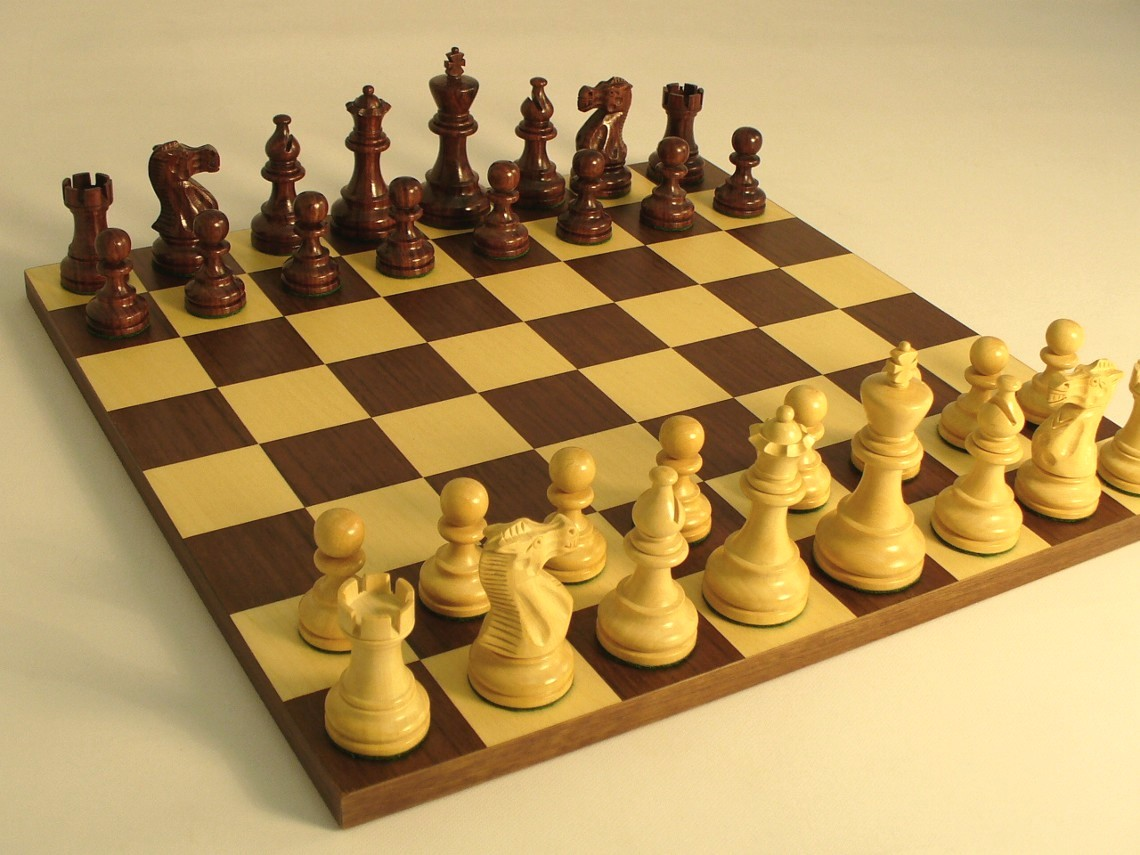
\includegraphics[width=0.7\linewidth]{chessboard.jpg}
\end{center}
\end{frame}

\begin{frame}
\frametitle{What do we know already?  The particles:}
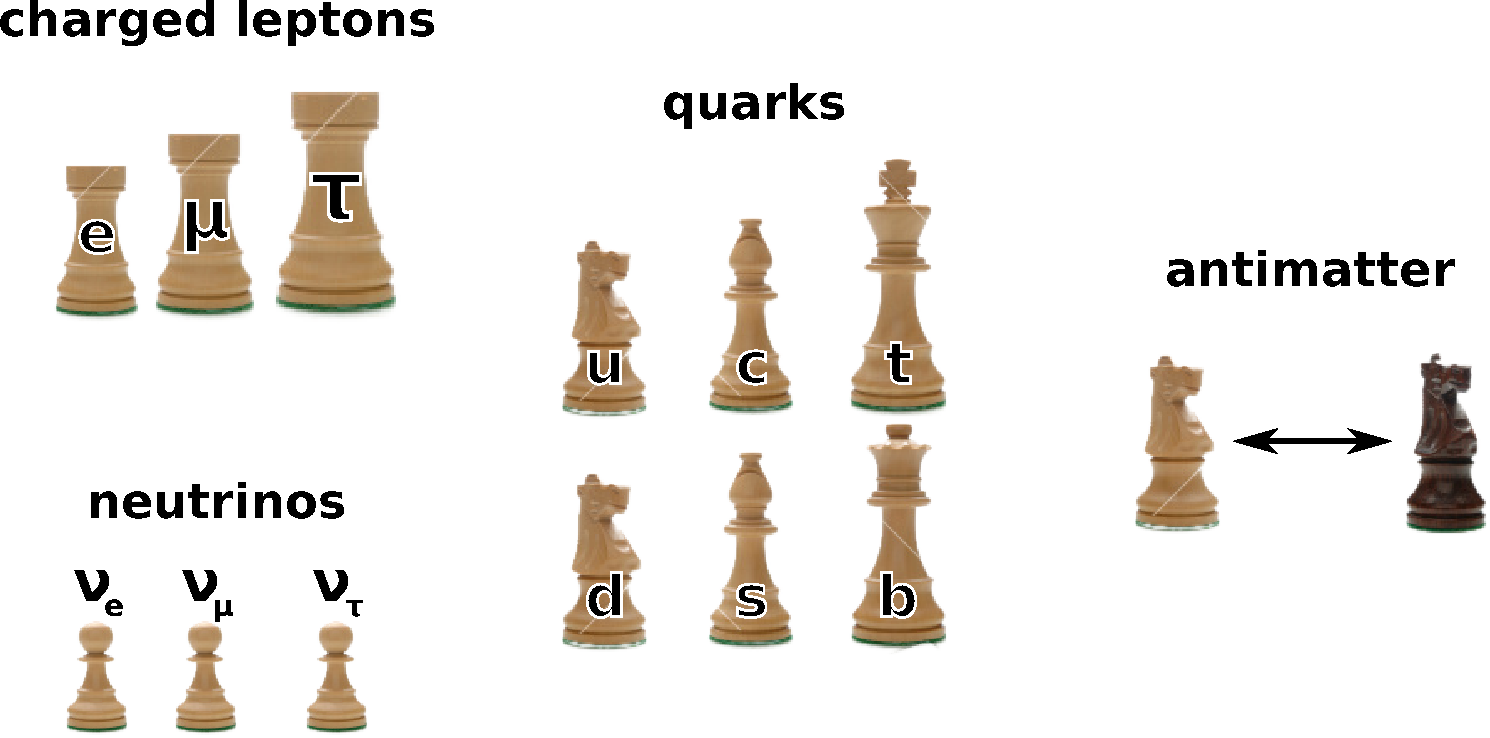
\includegraphics[width=\linewidth]{players.pdf}
\end{frame}

\begin{frame}
\frametitle{The electromagnetic force:}
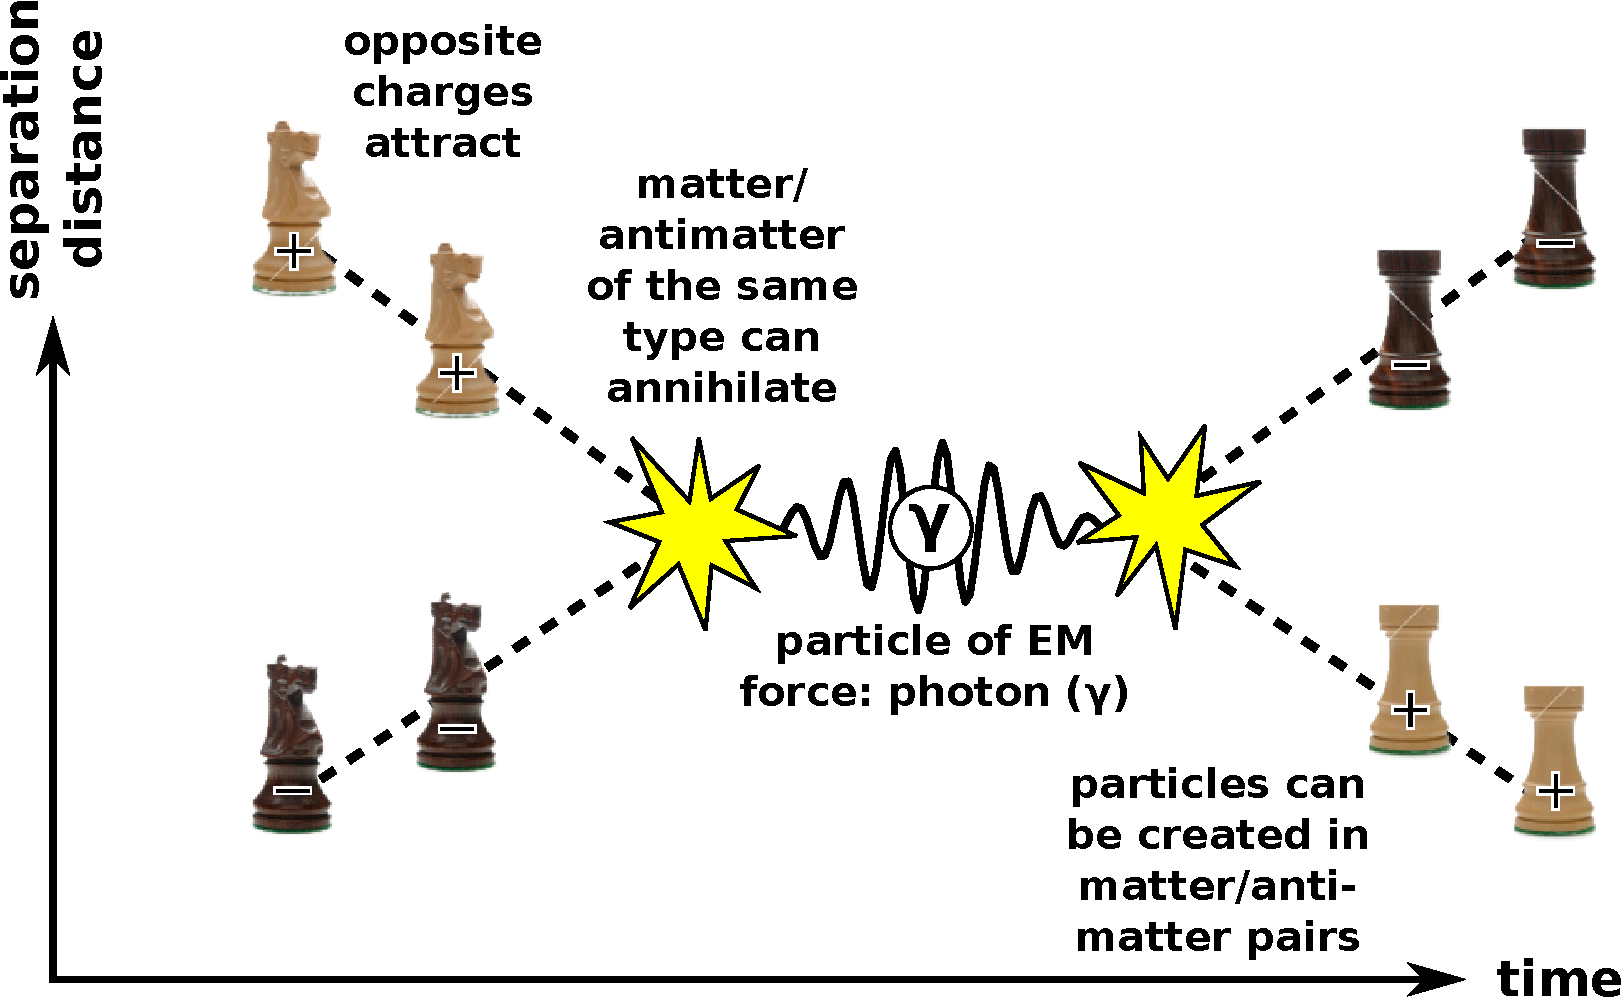
\includegraphics[width=\linewidth]{electromagnetism.pdf}
\end{frame}

\begin{frame}
\frametitle{The nuclear force:}
\begin{center}
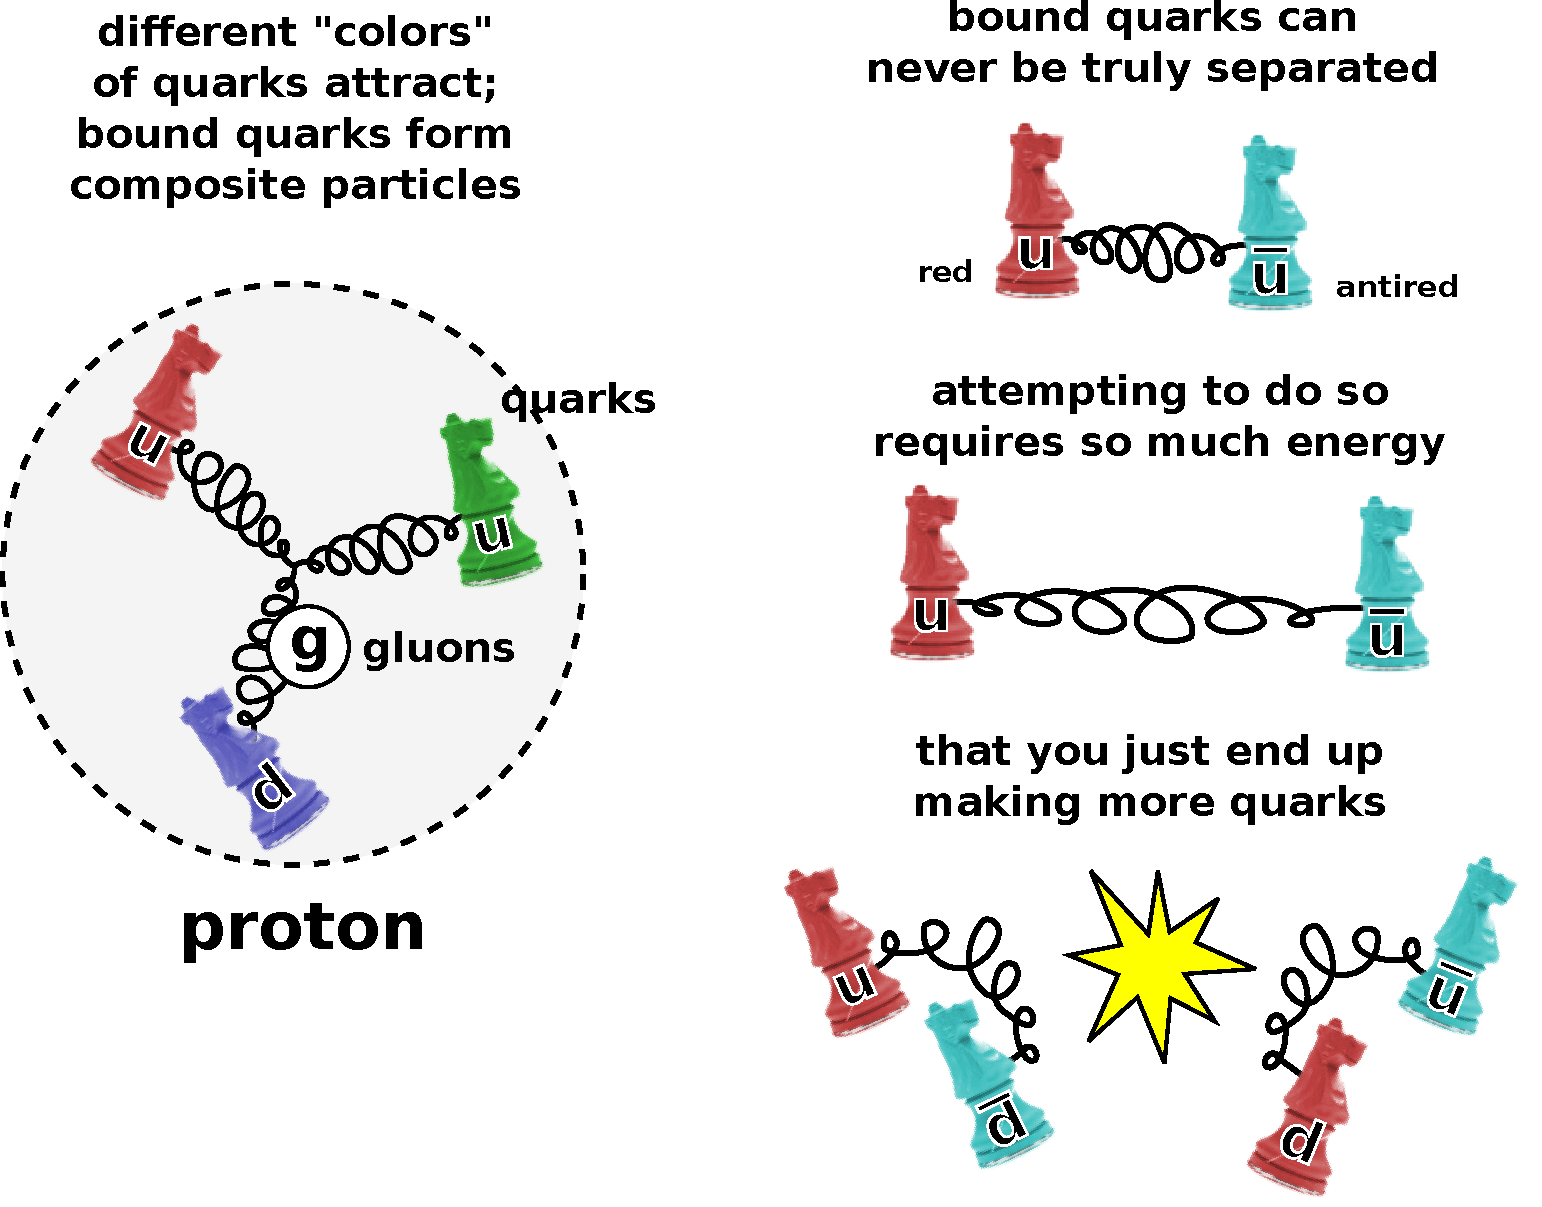
\includegraphics[width=0.95\linewidth]{nuclear.pdf}
\end{center}
\end{frame}

\begin{frame}
\frametitle{The weak interaction:}
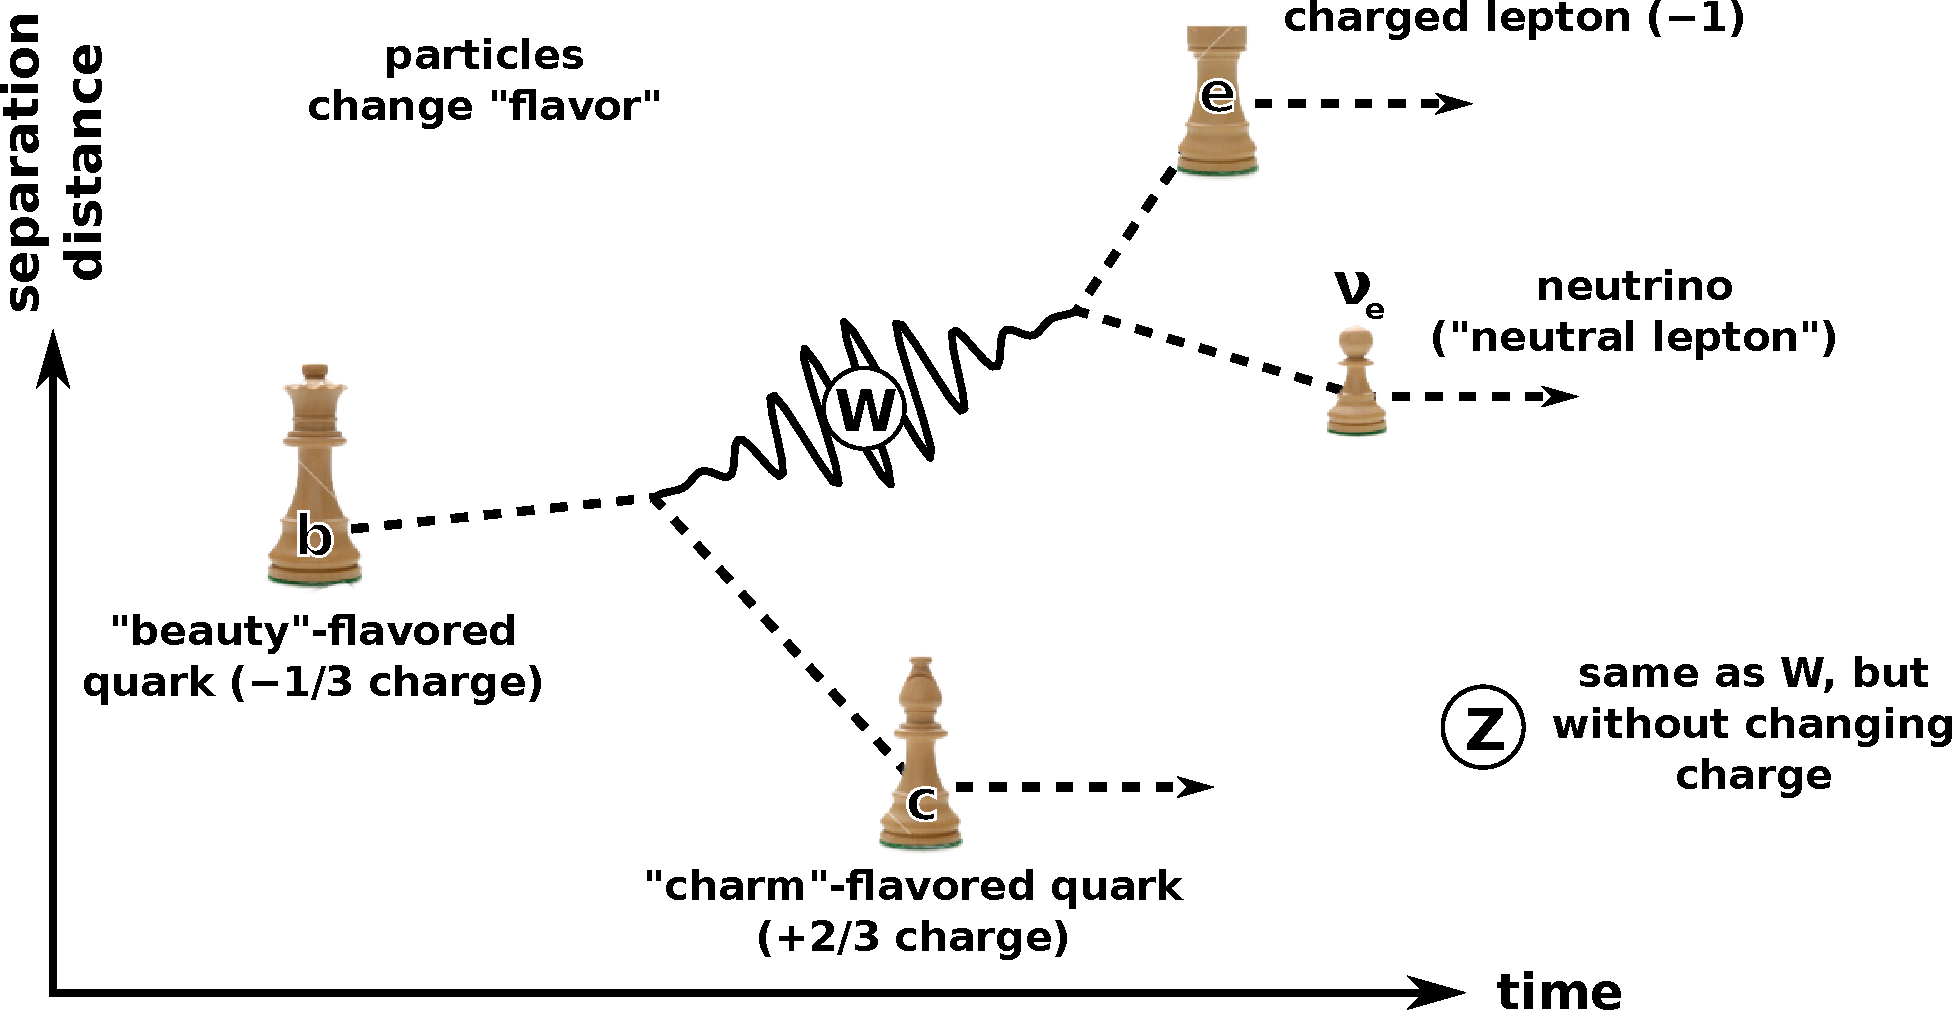
\includegraphics[width=\linewidth]{weakinteraction.pdf}
\end{frame}

\begin{frame}
\frametitle{Is this all?  How did we get here?}
\begin{center}
\large The Standard Model of Particle Physics
\end{center}
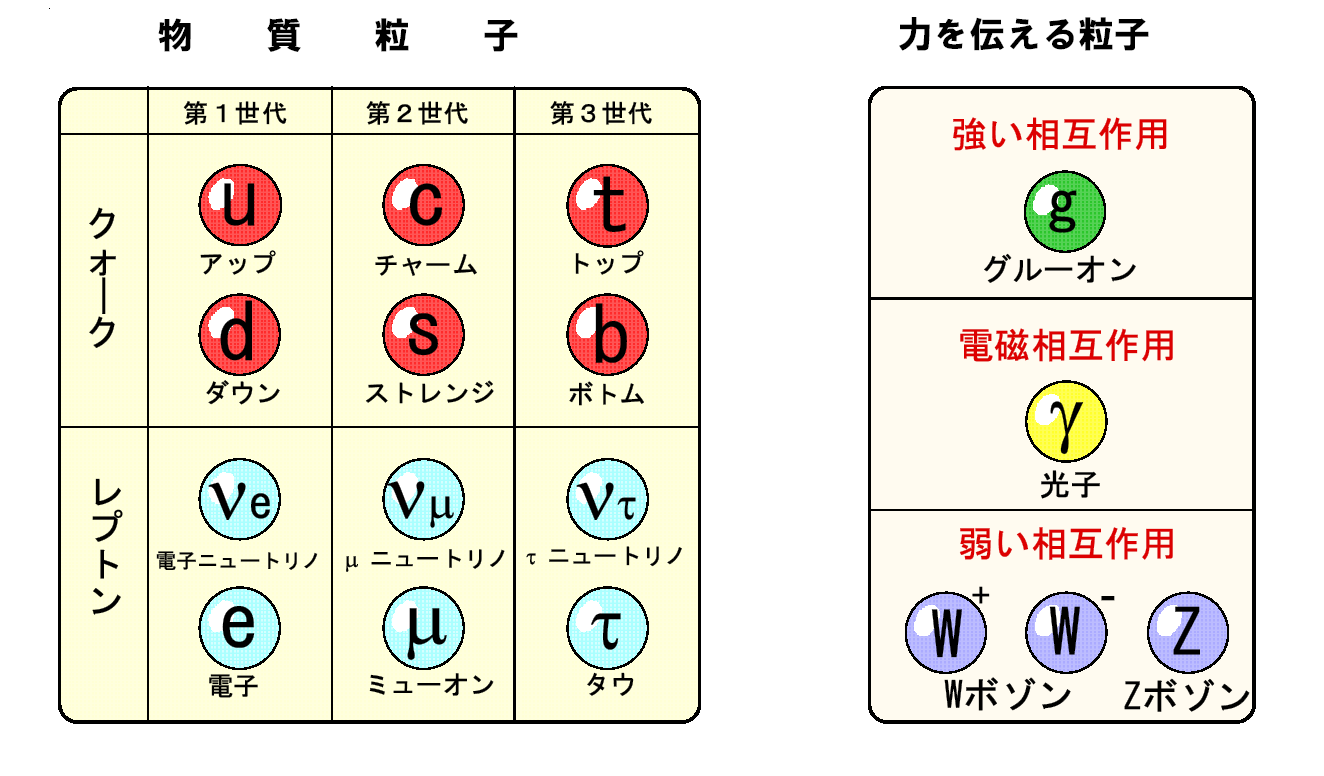
\includegraphics[width=\linewidth]{standard_model.png}
\end{frame}

\begin{frame}
\frametitle{Timeline 1: everything settles into place}
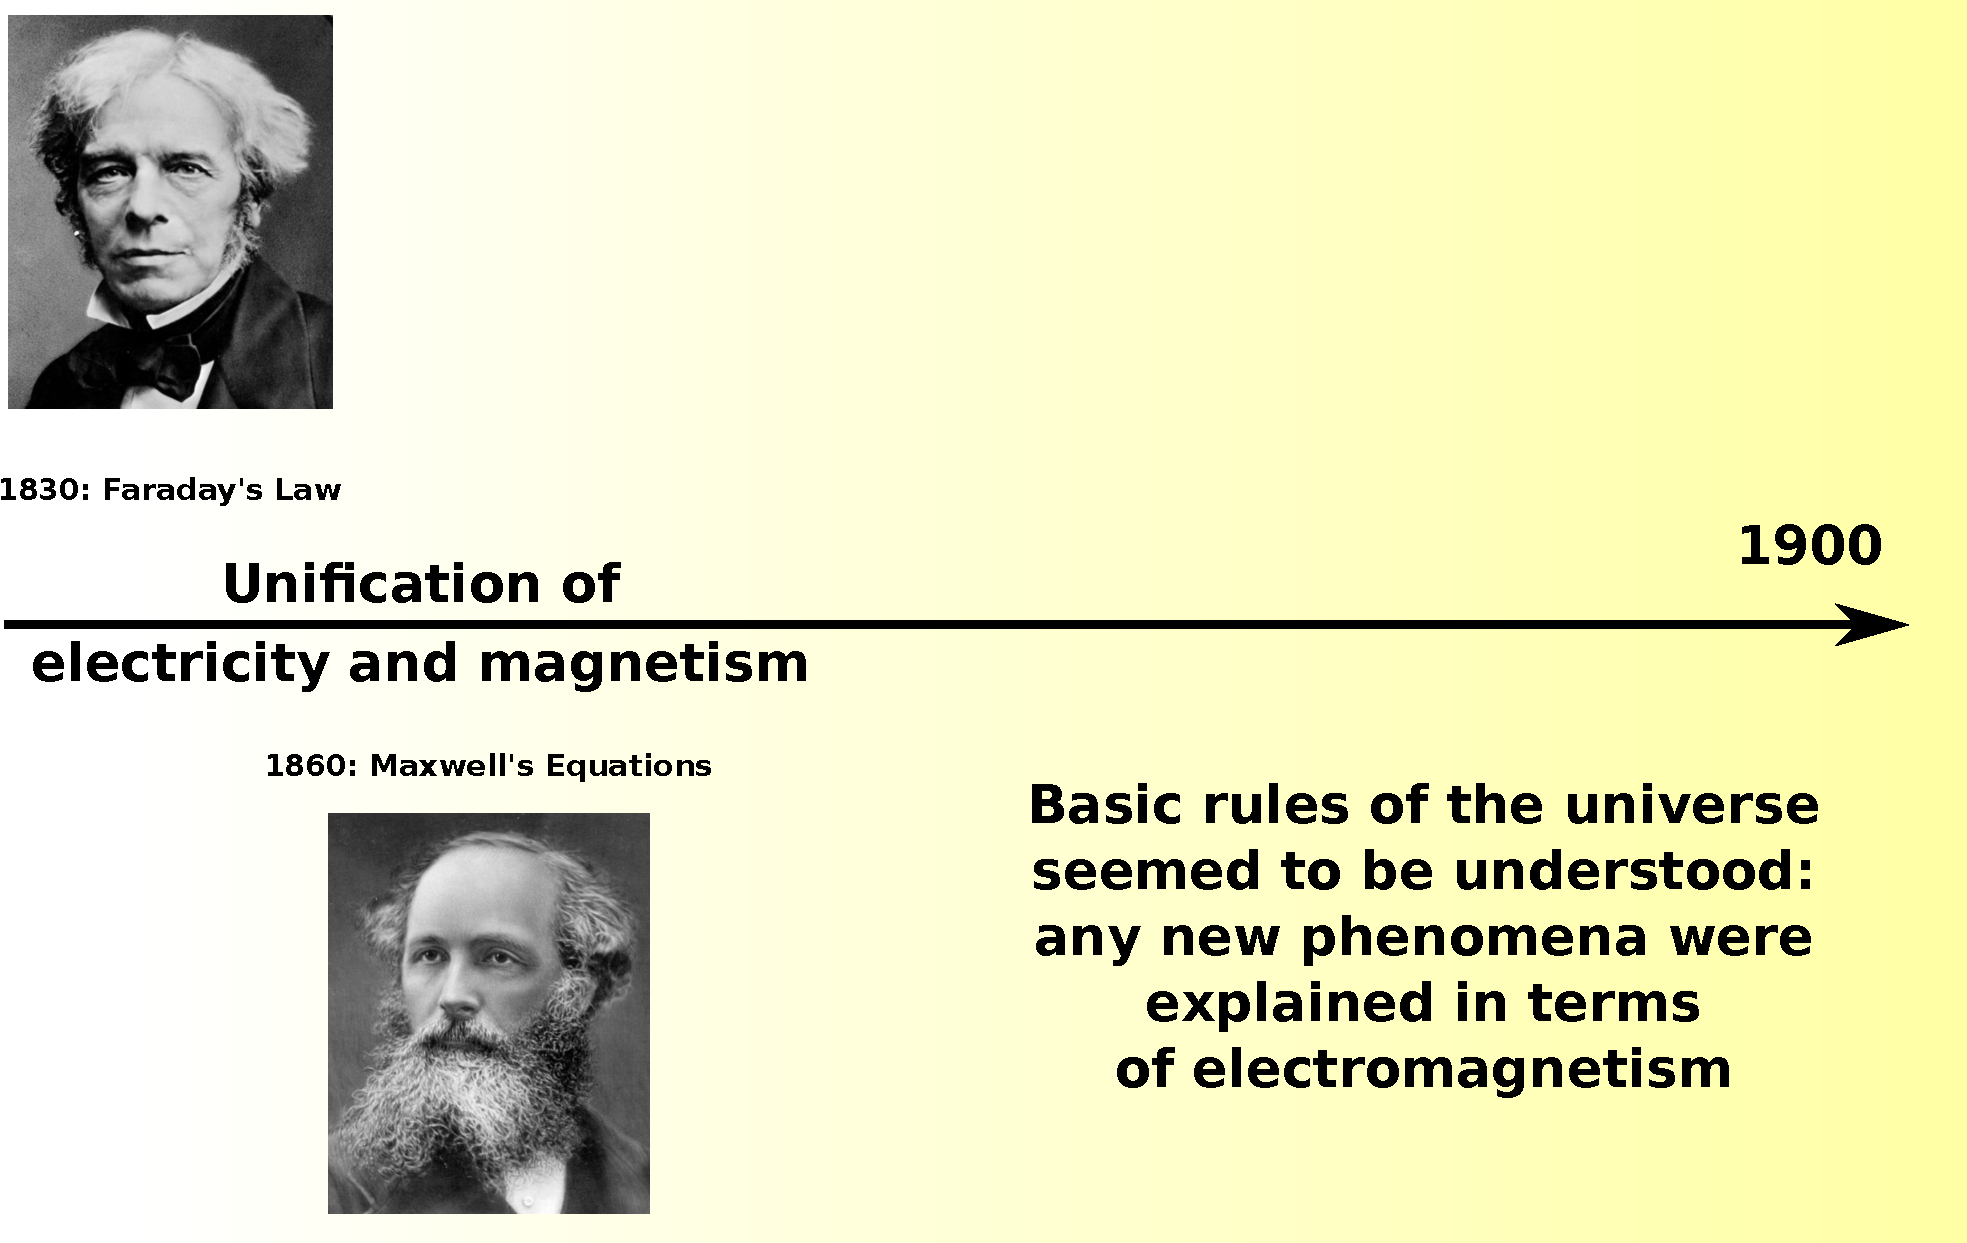
\includegraphics[width=\linewidth]{timeline1.pdf}
\end{frame}

\begin{frame}
\frametitle{Timeline 2: everything jumps out of place!}
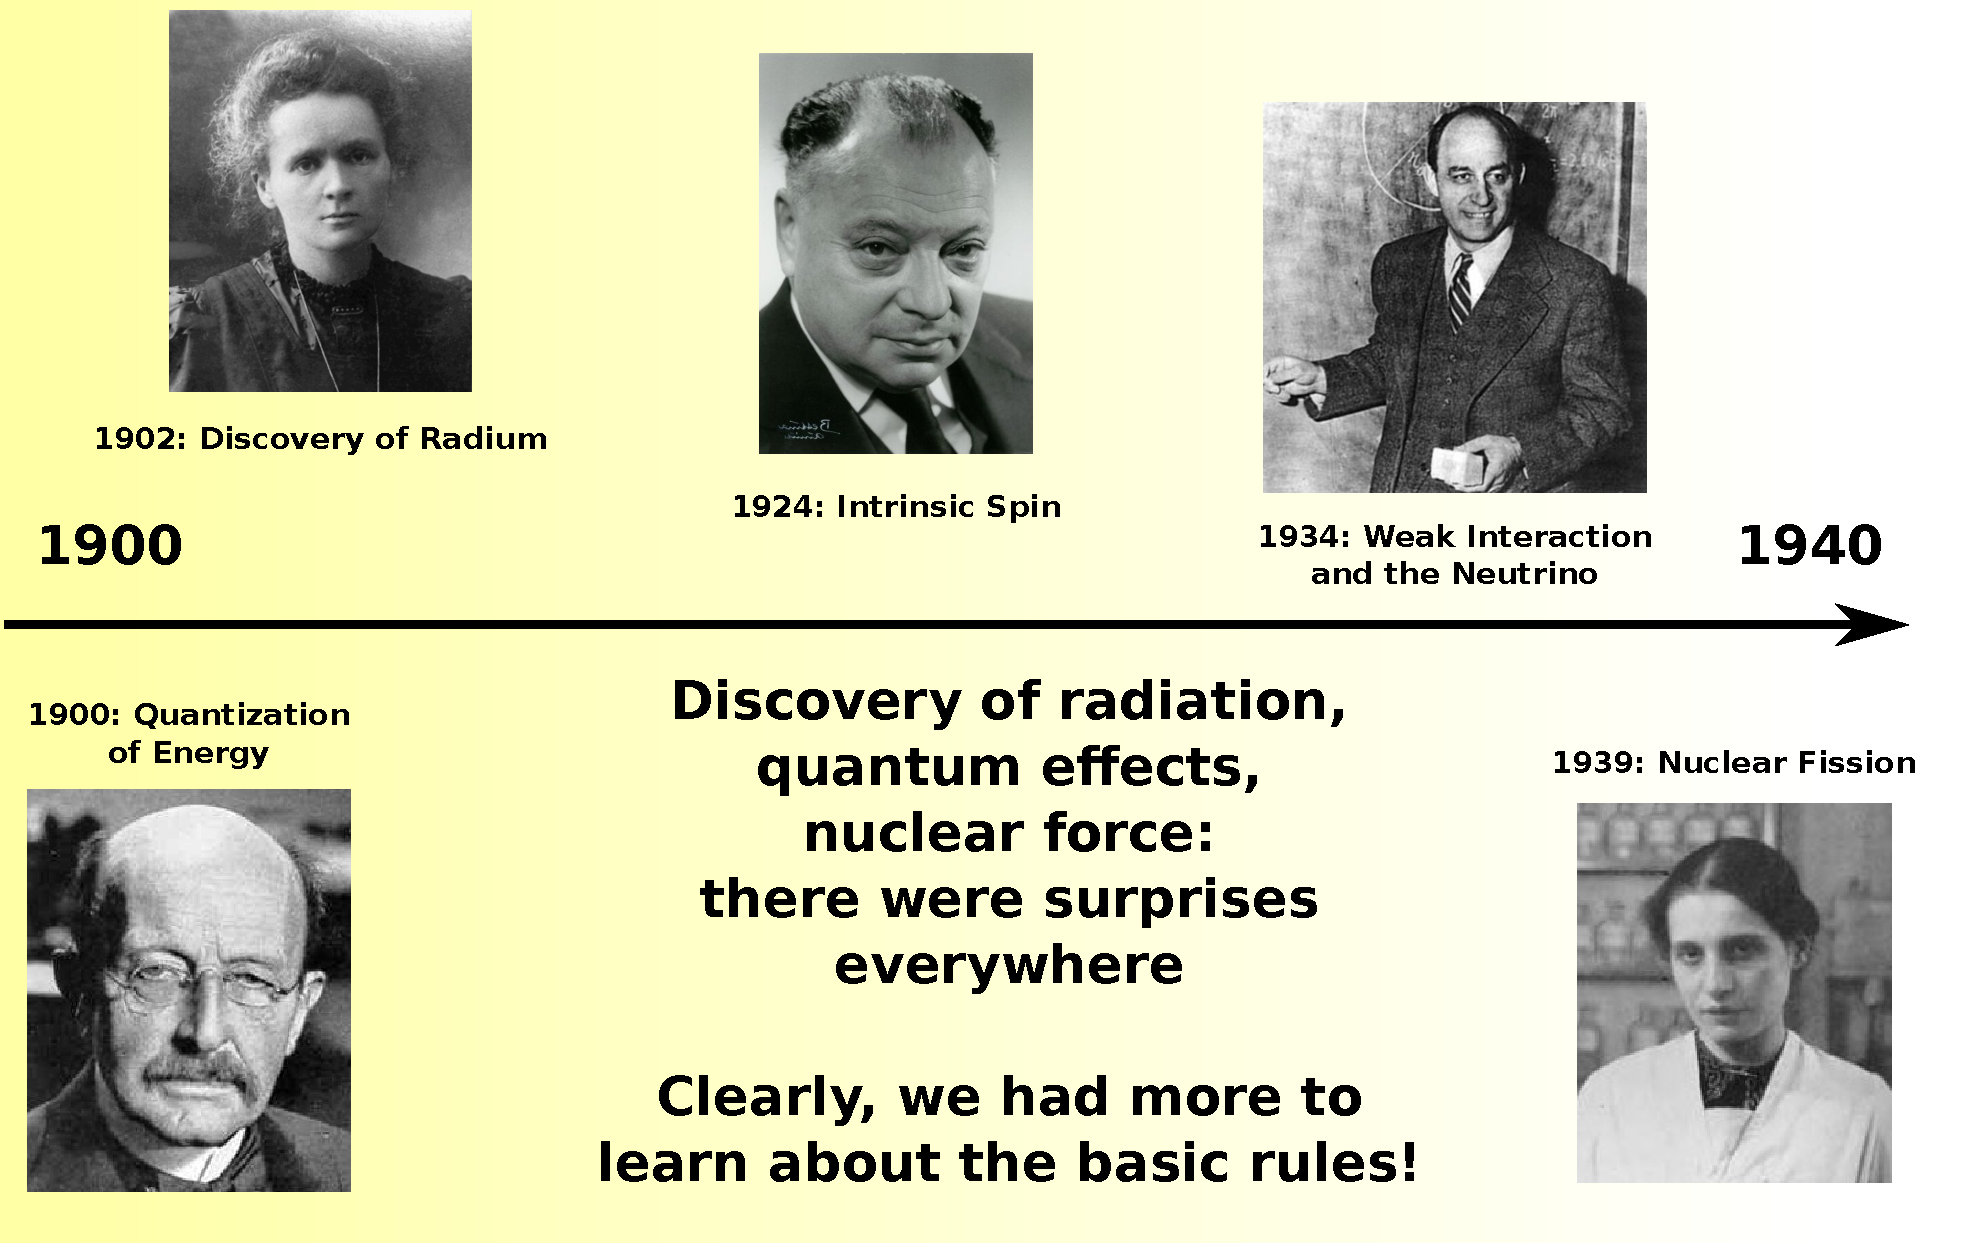
\includegraphics[width=\linewidth]{timeline2.pdf}
\end{frame}

\begin{frame}
\frametitle{Timeline 3: everything starts settling again}
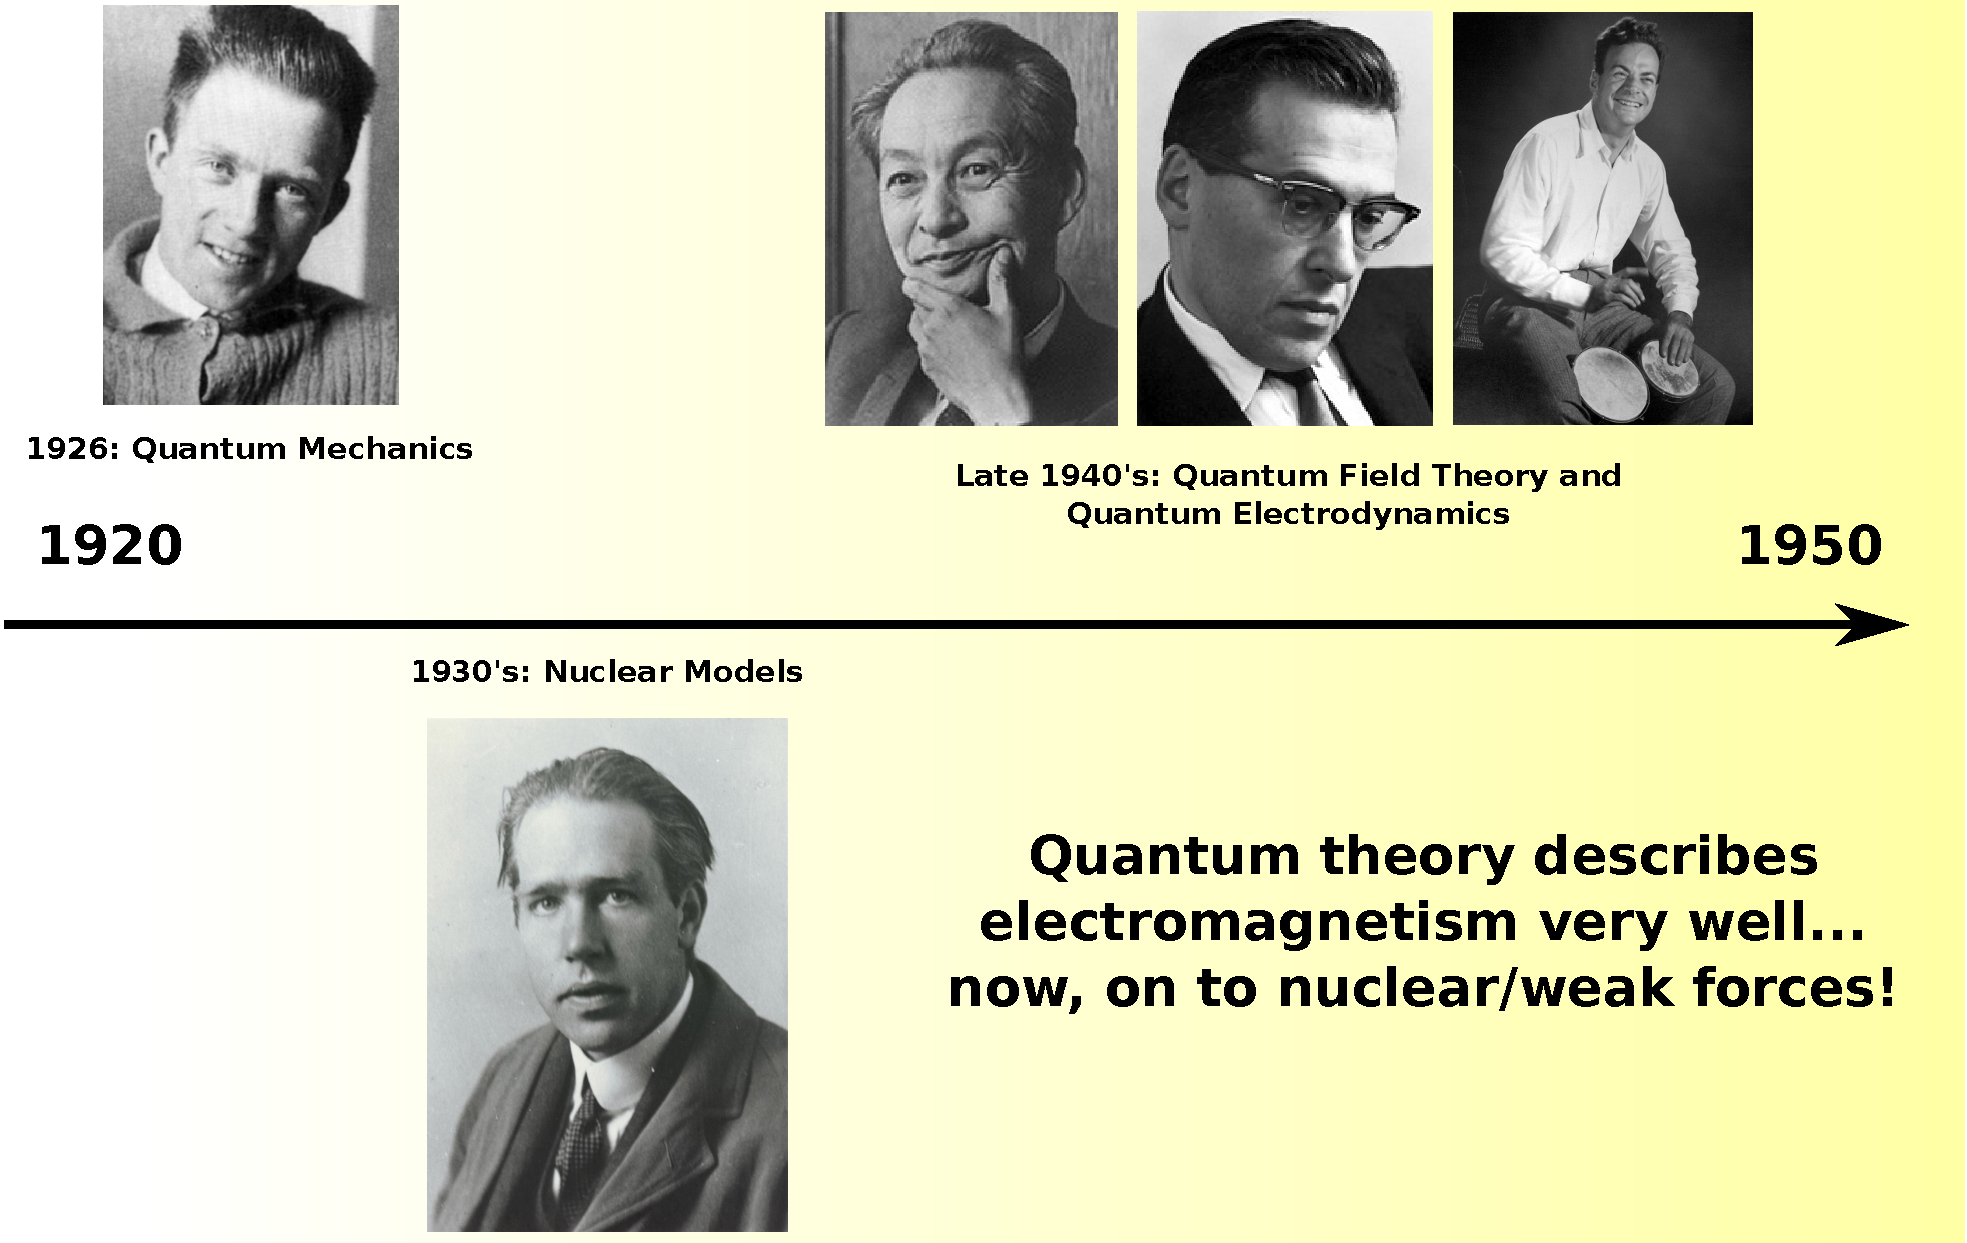
\includegraphics[width=\linewidth]{timeline3.pdf}
\end{frame}

\begin{frame}
\frametitle{Timeline 4: everything gets more complex}
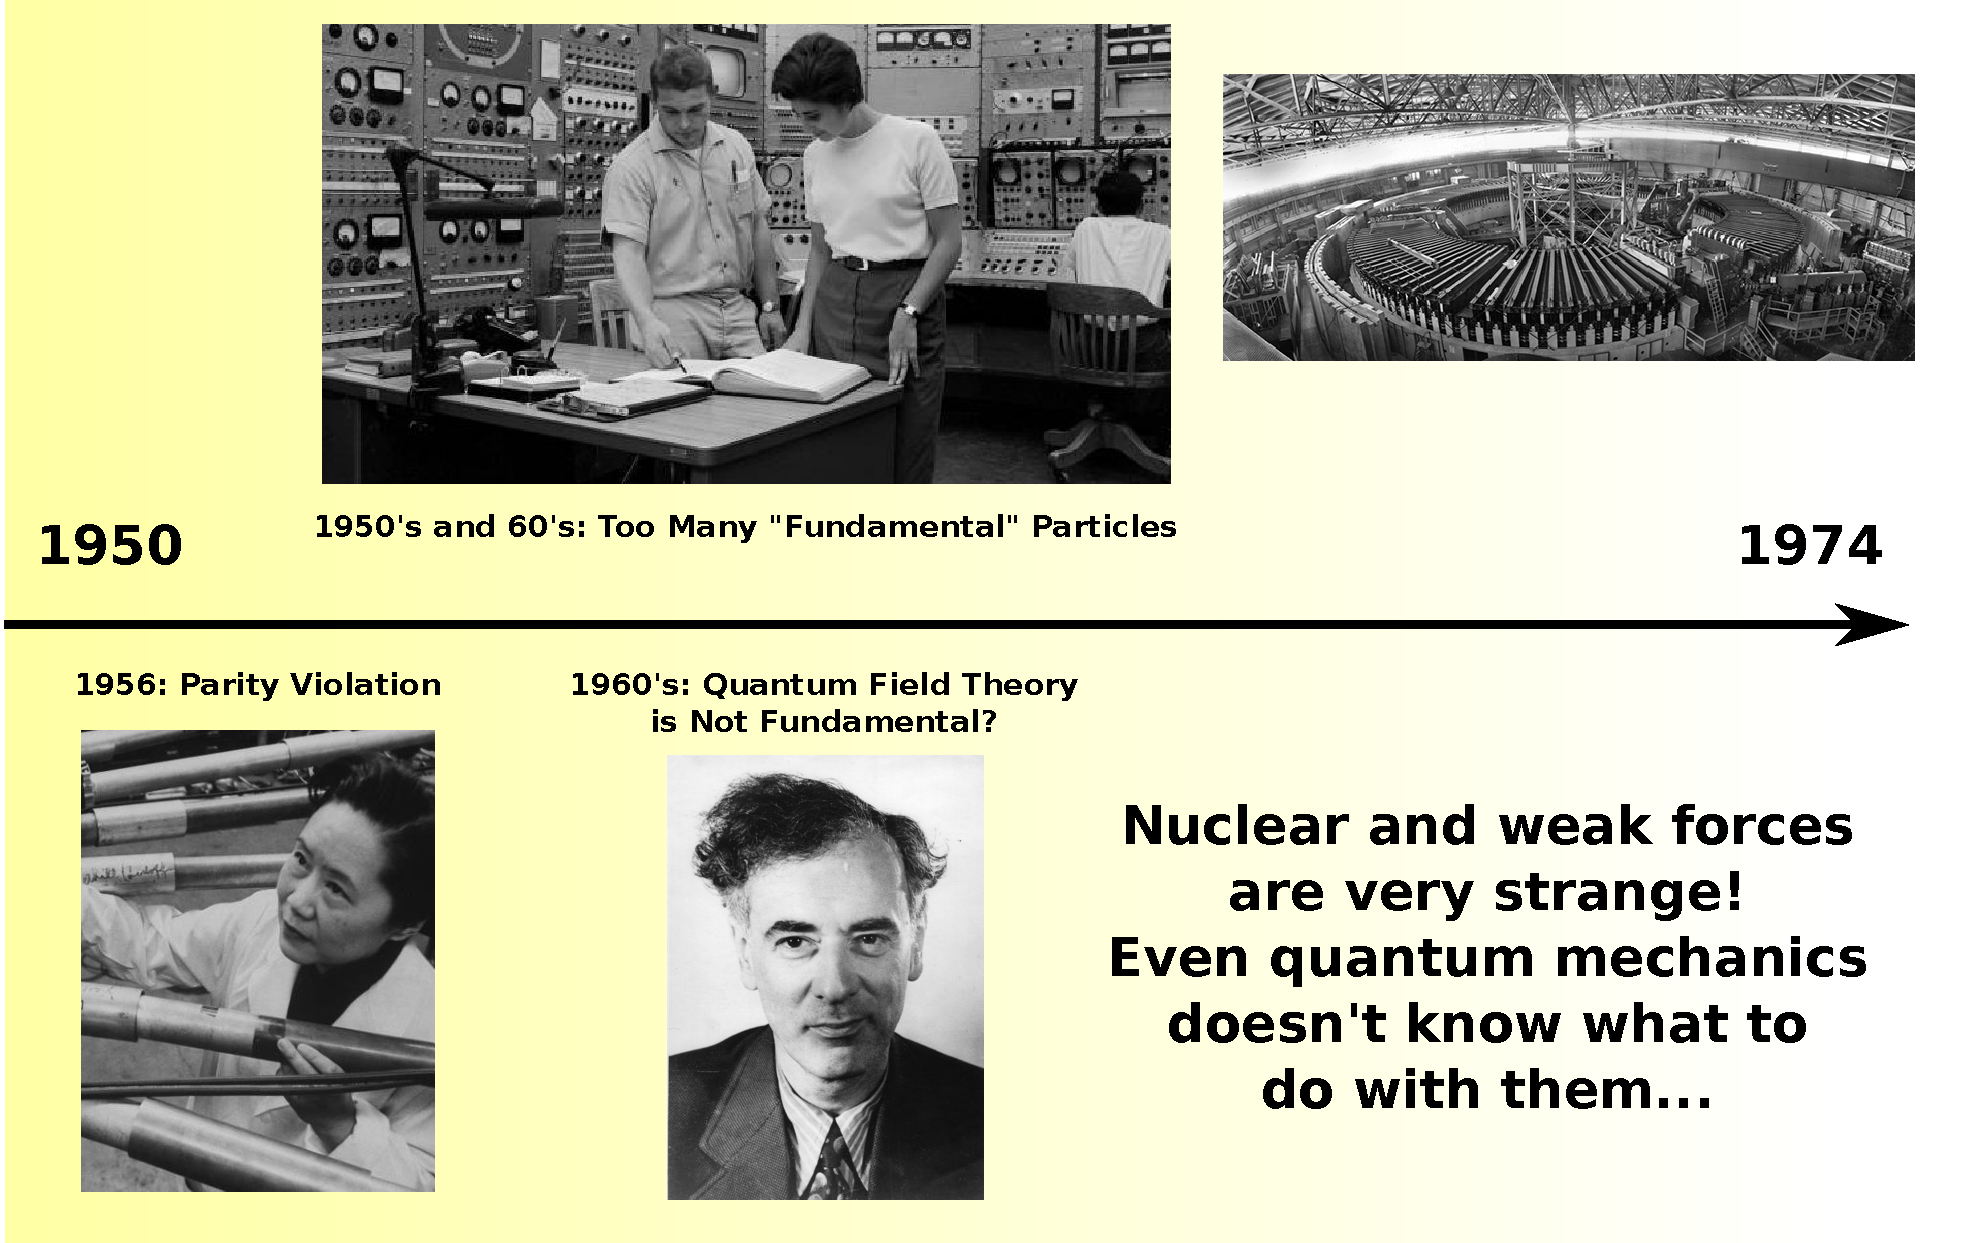
\includegraphics[width=\linewidth]{timeline4.pdf}
\end{frame}

\begin{frame}
\frametitle{Timeline 5: it all makes sense again!}
\framesubtitle{\ldots\ or does it?}
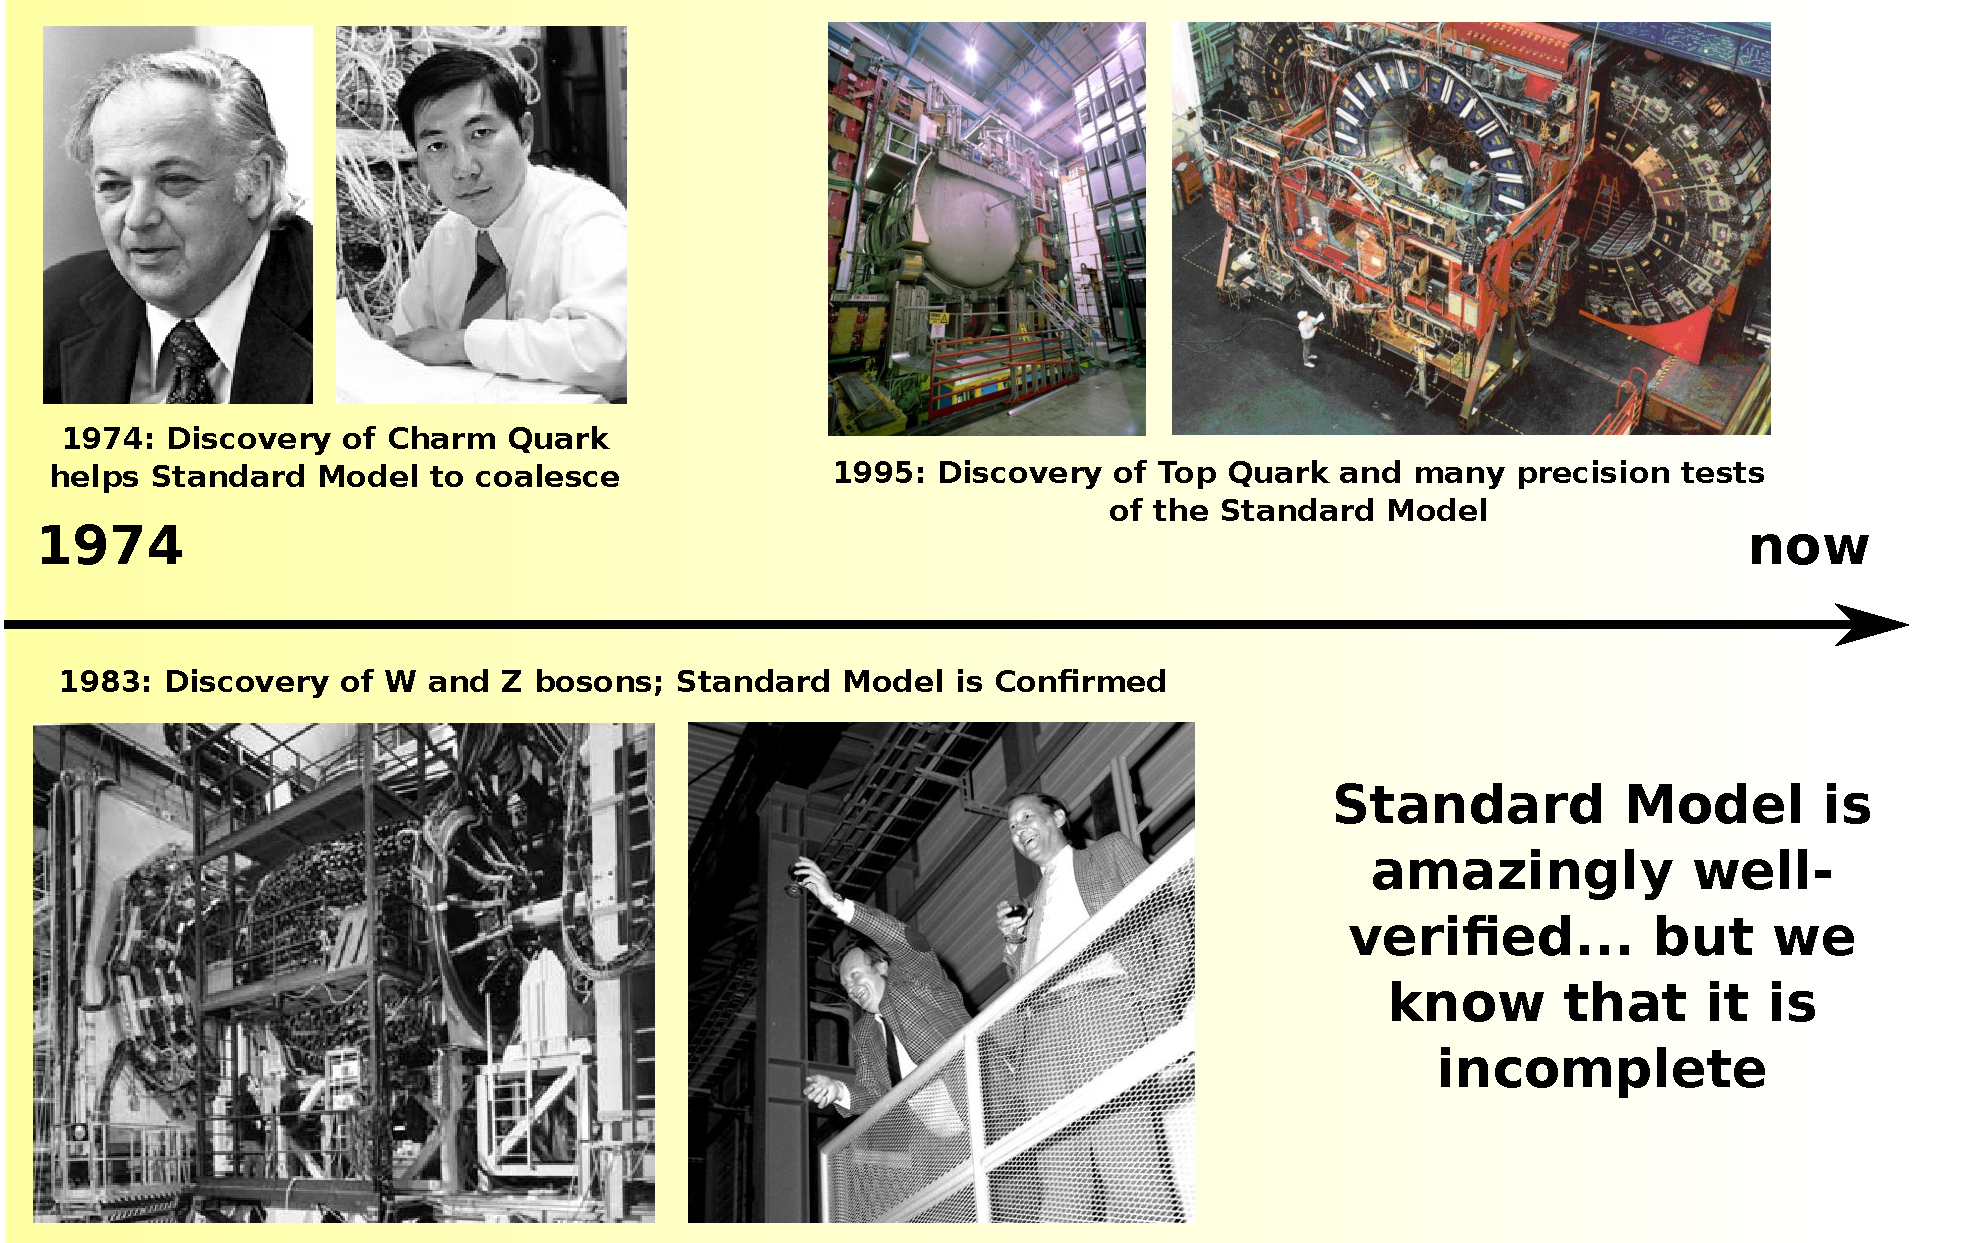
\includegraphics[width=\linewidth]{timeline5.pdf}
\end{frame}

\begin{frame}
\frametitle{\#1: The Standard Model {\it needs} a Higgs}

Couplings between particles (matter and forces):
\begin{center}
\only<1-2>{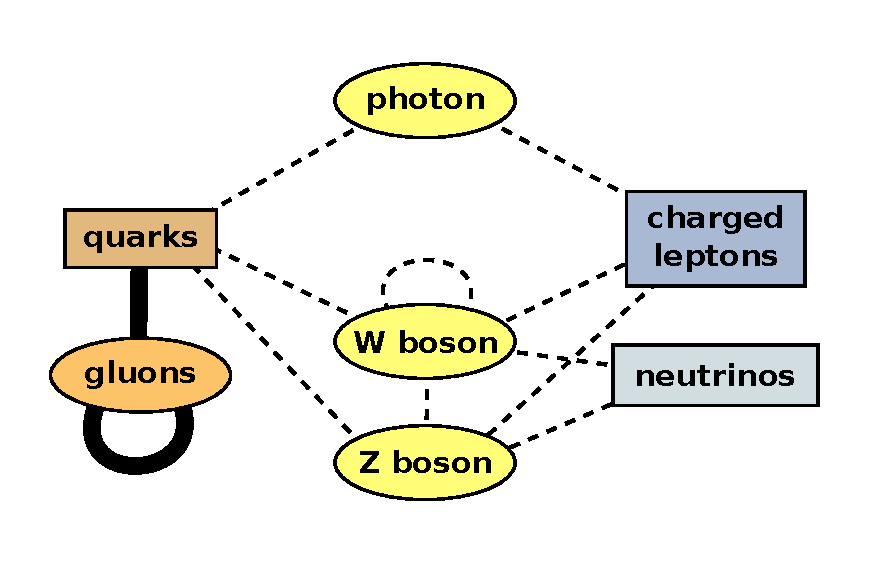
\includegraphics[width=0.75\linewidth]{standard_model.pdf}}
\only<3>{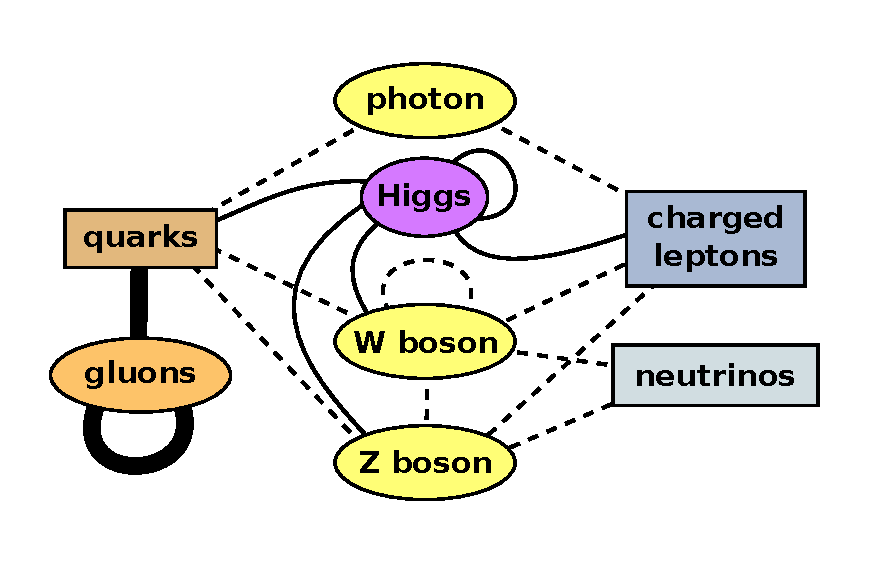
\includegraphics[width=0.75\linewidth]{standard_model_whiggs_quarkmass.pdf}}
\end{center}

\vspace{-1 cm}
\begin{itemize}
\item<2-3> Force particles cannot have mass in the fundamental theory
\item<2-3> $W$ and $Z$ have very large masses, in apparent contradiction
\item<3> Their masses can be dynamically generated by interacting with another field: the Higgs boson
\end{itemize}
\end{frame}

\begin{frame}
\frametitle{But where is it?}

\begin{itemize}
\item From $W$, $Z$, and top quark masses, best-fit Higgs mass should be 80~GeV
\item Higgs mass below 114 GeV and between 160--170 GeV are ruled out by experiment
\item The whole picture is possible, but increasingly unlikely as more
  possibilities are ruled out
\end{itemize}

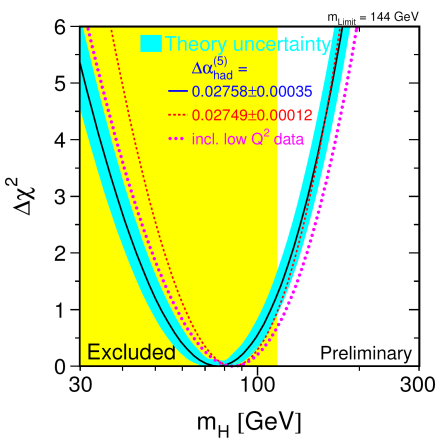
\includegraphics[height=4.3 cm]{higgsMass.png} \hfill
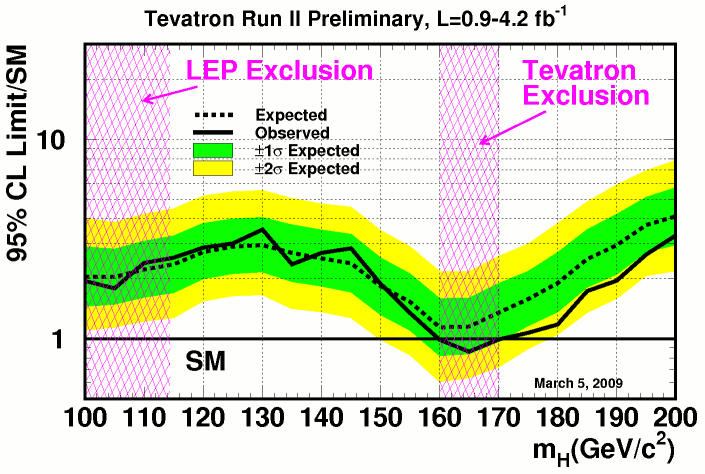
\includegraphics[height=4.3 cm]{fermilab_higgs_exclusion.png}
\end{frame}

\begin{frame}
\frametitle{\#2: The Standard Model is unnatural}

\begin{itemize}
\item The Standard Model does not include quantum gravity
\begin{itemize}
\item somehow, it needs to fit into a larger theory that does \\ (string theory?)
\end{itemize}
\item The connection between the Standard Model and a fully unified theory is awkward:
\begin{itemize}
\item no explanation why Higgs mass would be as light as it needs \mbox{to be\hspace{-1 cm}}
\item doesn't properly unify electromagnetic, nuclear, and weak forces at high energy
\end{itemize}
\item Very likely, there is another piece to the puzzle between the
  Standard Model and quantum gravity
\end{itemize}
\end{frame}

\begin{frame}
\frametitle{Supersymmetry}
\begin{itemize}
\item Introducing a new relationship between matter particles and
  force particles solves both problems
\item Also provides us with a lot more particles to discover!
\end{itemize}

\begin{center}
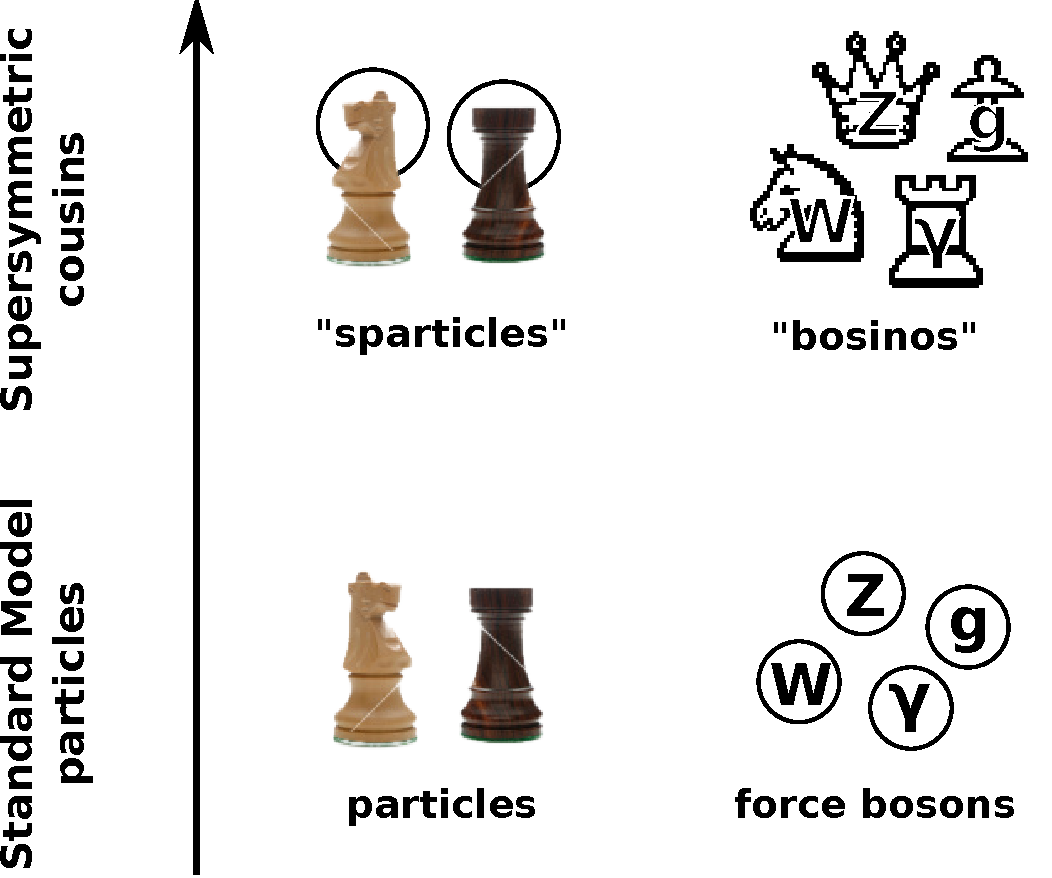
\includegraphics[width=0.65\linewidth]{supersymmetry.pdf}
\end{center}
\end{frame}

\begin{frame}
\frametitle{\#3: We know there's other stuff out there}
\begin{columns}
\column{0.5\linewidth}
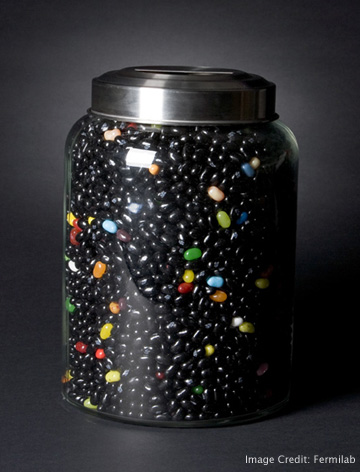
\includegraphics[width=\linewidth]{darkmatter.jpg}

\column{0.5\linewidth}
Astronomers have determined the following composition of the universe from recent measurements:
\begin{itemize}
\item 0.03\% of it is heavy elements (anything solid, like us)
\item 0.3\% neutrinos
\item 0.5\% stars
\item 4\% free-floating H, He gasses
\item 25\% some new kind of particle, {\it not in the Standard Model} (``dark matter'')
\item 70\% something else, not even particle-like (``dark energy'')
\end{itemize}
\end{columns}
\end{frame}

%% \begin{frame}
%% \frametitle{Outline}
%% \begin{itemize}\setlength{\itemsep}{0.75 cm}
%% \item 
%% \end{itemize}
%% %% \hspace{-0.83 cm} \textcolor{darkblue}{\Large Outline2}
%% \end{frame}

%% \section*{First section}
%% \begin{frame}
%% \begin{center}
%% \Huge \textcolor{blue}{First section}
%% \end{center}
%% \end{frame}

\begin{frame}
\frametitle{What to do about it: TeV-scale colliders!}

From {\it Popular Mechanics,} 1978; immediately after the Standard
Model was formulated and its implications realized

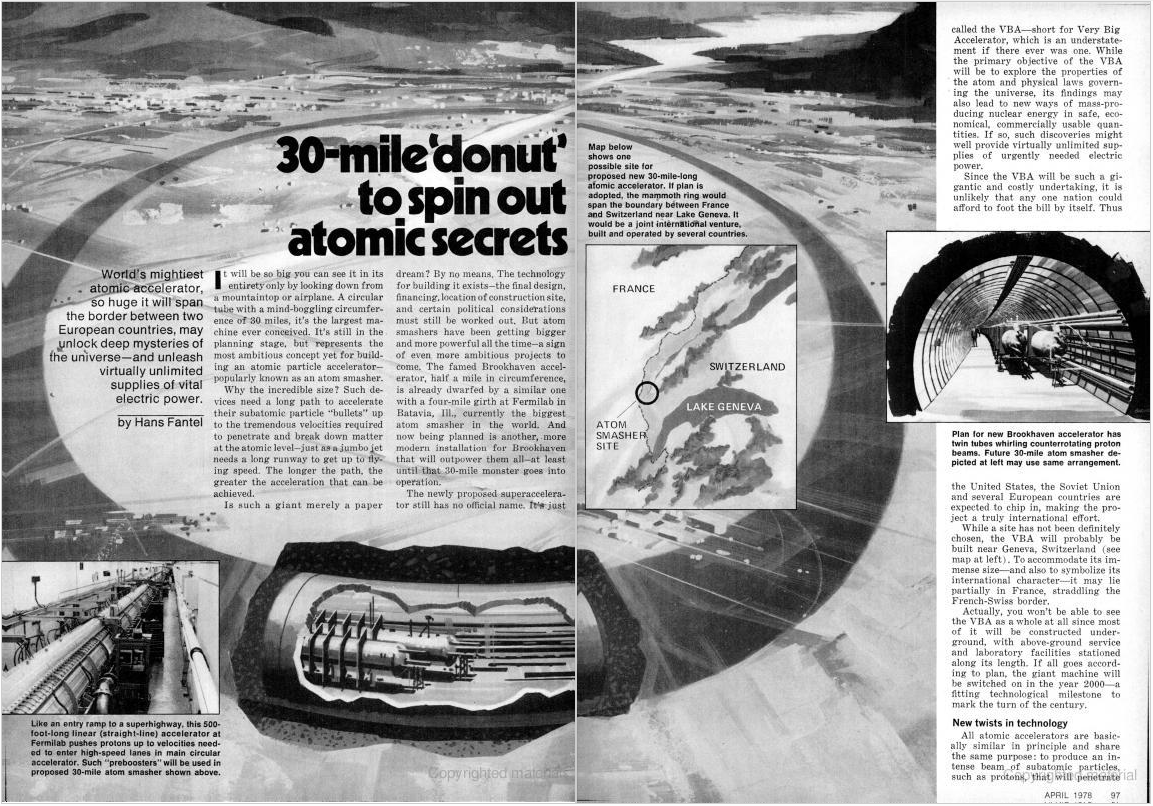
\includegraphics[width=\linewidth]{popular_mechanics.png}
\end{frame}

\begin{frame}
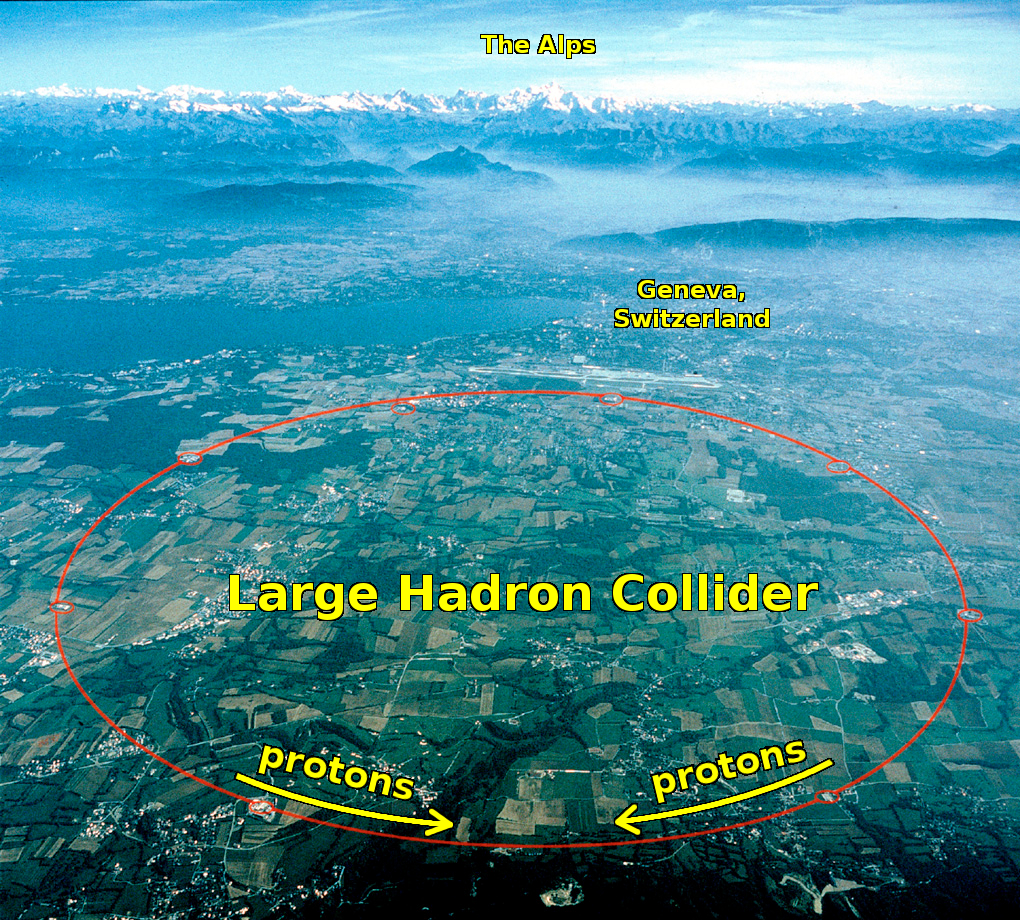
\includegraphics[width=0.9\linewidth]{cernpanorama.jpg}
\end{frame}

\begin{frame}
\frametitle{Hopefully, we'll soon be confused again}
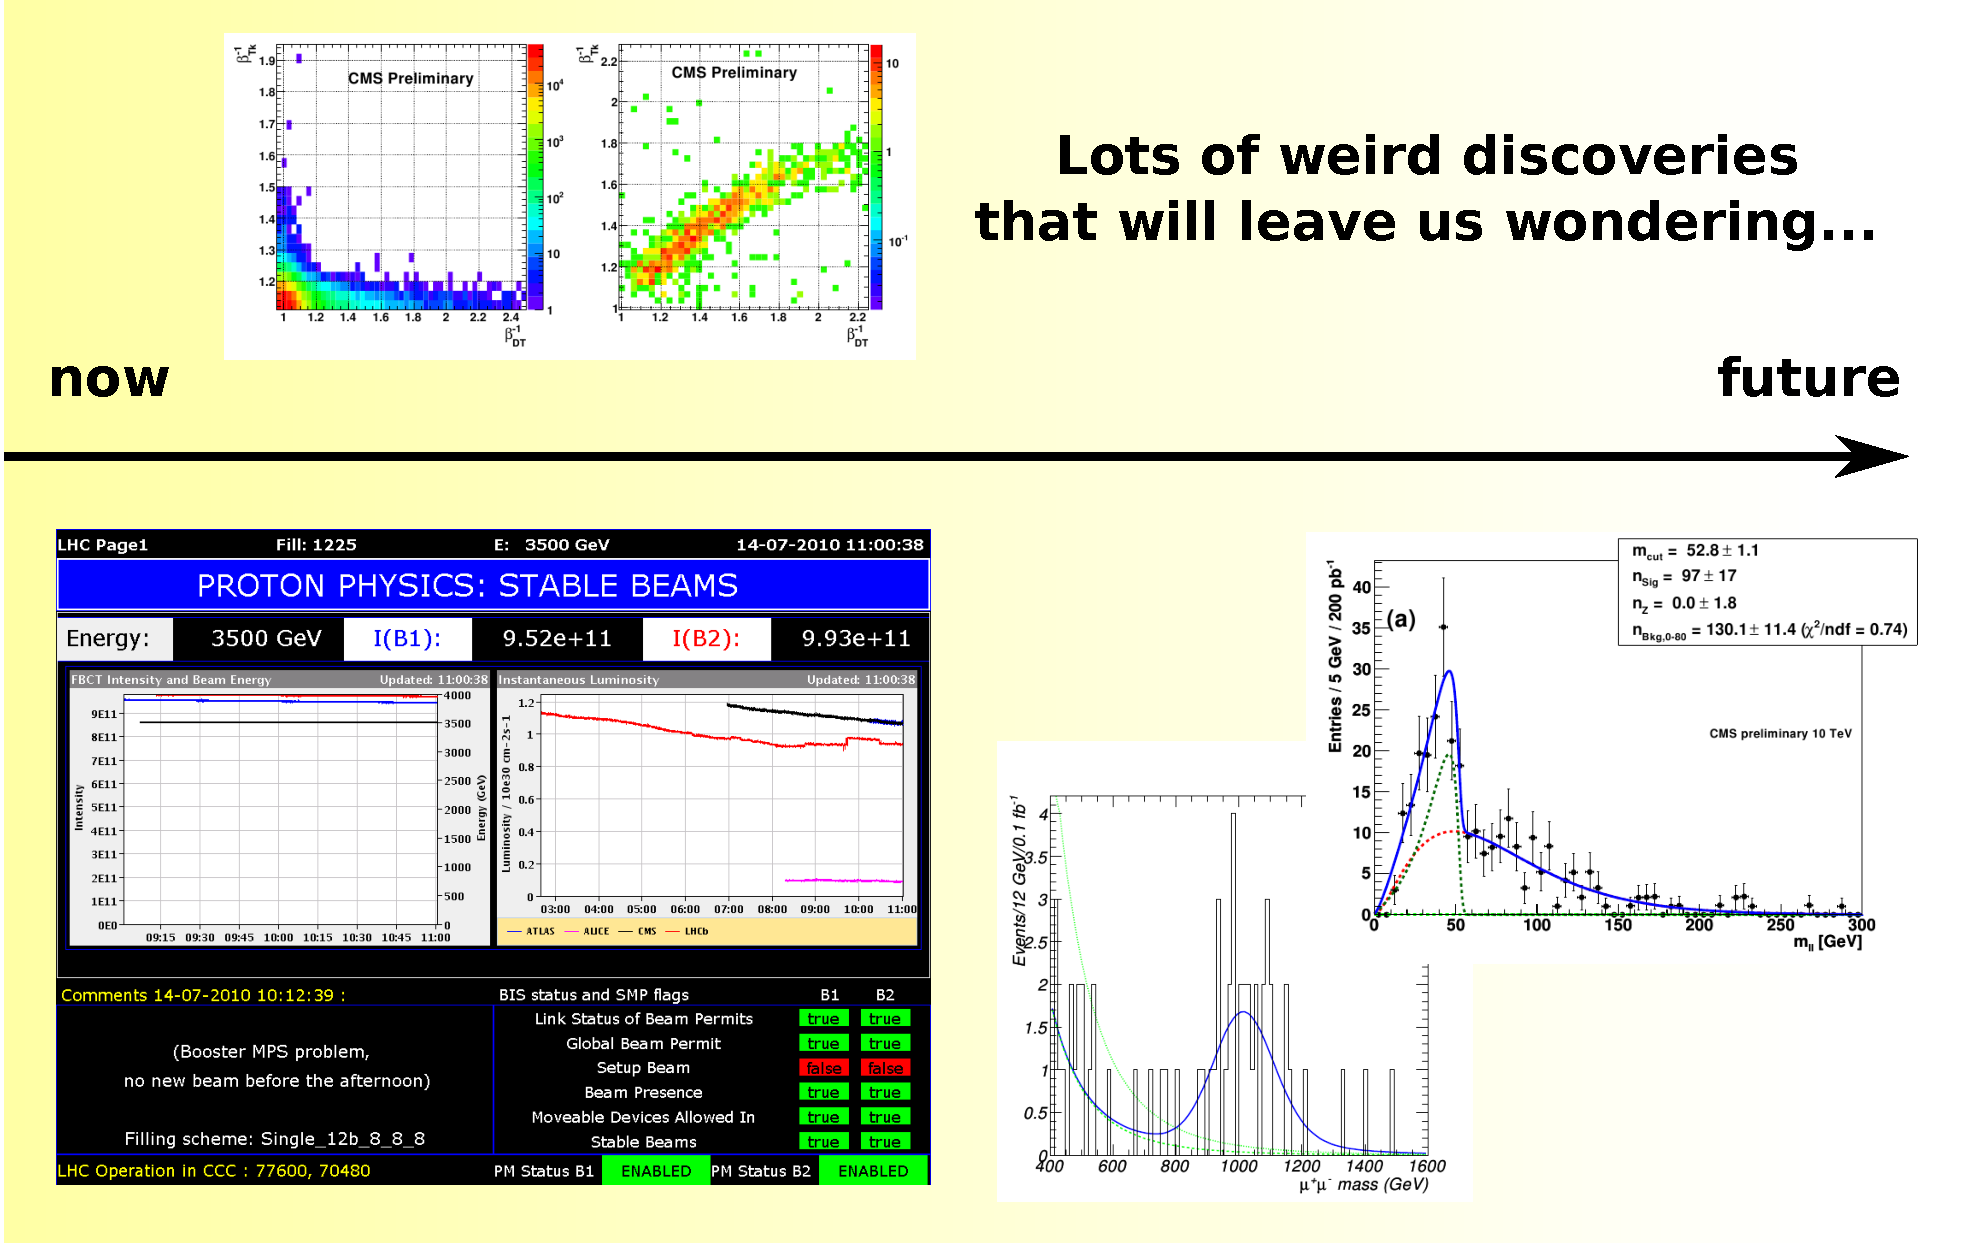
\includegraphics[width=\linewidth]{timeline6.pdf}
\label{numpages}
\end{frame}

\end{document}
